\documentclass{beamer}
\usepackage{amsfonts}
\usepackage{amsmath}
\usepackage{amssymb}
\usepackage{amsthm}
\usepackage{bm}
\usepackage{booktabs}
\usepackage{dsfont}
\usepackage{caption}
\usepackage{enumerate}
\usepackage{fancyhdr}
\usepackage{float}
\usepackage{graphicx}
\usepackage{natbib}
\usepackage{pifont}
% \usepackage[section]{placeins} % to make figures stay at the same section
\usepackage{soul}
\usepackage{subcaption}
\usepackage{tikz}
% \usepackage[margin=1in]{geometry}

\usepackage{xcolor}


\DeclareMathOperator{\e}{e}
\DeclareMathOperator{\cov}{Cov}
\DeclareMathOperator{\corr}{Corr}
\DeclareMathOperator{\var}{Var}
\DeclareMathOperator{\expect}{\ensuremath{\mathbb{E}}}
\DeclareMathOperator{\Log}{Log}
\DeclareMathOperator*{\res}{Res}
\DeclareMathOperator{\re}{Re}
\DeclareMathOperator{\im}{Im}
\DeclareMathOperator{\Arg}{Arg}
\DeclareMathOperator{\conv}{conv}
\DeclareMathOperator{\tr}{tr}
\newcommand\dif{\ensuremath{\mathrm{d}}}
\newcommand\prob{\ensuremath{\mathbb{P}}}
\newcommand\real{\ensuremath{\mathbb{R}}}
\newcommand\sigmaf{\ensuremath{\mathcal{F}}}
\newcommand\sigmag{\ensuremath{\mathcal{G}}}
\newcommand\sigmah{\ensuremath{\mathcal{H}}}
\newcommand\gaussian{\ensuremath{\mathcal{N}}}
\newcommand\lagrange{\ensuremath{\mathcal{L}}}
\newcommand\fisher{\ensuremath{\mathcal{I}}}
\newcommand\converge[1]{\ensuremath{\rightarrow_{#1}}}
\newcommand\convergeas{\converge{\text{a.s.}}}
\newcommand\convergep{\converge{\prob}}
\newcommand\convergedist{\converge{\text{d}}}
\newcommand\convergelp{\converge{\mathcal{L}_p}}
\newcommand\loss{\ensuremath{\mathcal{L}}}
\newcommand\crlb{\ensuremath{\text{CRLB}}}
\newcommand\todo{\textcolor{red}{\textbf{TODO}}}
\newcommand{\tick}{\ding{51}}
\newcommand*\indicator[1]{\ensuremath{\mathds{1}\left\{#1\right\}}}
\newcommand*\abs[1]{\ensuremath{\left\vert #1 \right\vert}}
\newcommand*\norm[1]{\ensuremath{\left\Vert #1 \right\Vert}}
\newcommand*\inner[1]{\ensuremath{\left\langle #1 \right\rangle}}
\newcommand*\T[1]{\ensuremath{{#1}^{\operatorname{T}}}}
\renewcommand*\vec[1]{\ensuremath{\bm{#1}}}
\renewcommand\emptyset{\ensuremath{\varnothing}}
\renewcommand\epsilon{\ensuremath\varepsilon}
% \renewcommand\phi{\ensuremath\varphi}

\usetheme{Boadilla}
\usecolortheme{seahorse}
\beamertemplatenavigationsymbolsempty




\bibliographystyle{plainnat}
\title{Generating Volatility Surfaces of Index Option with VAEs}
\author{Haoqiang Zhang, Siqing Zou, Zhuolin Xiang}
\date{\today}
\setbeamertemplate{footline}[frame number]
\begin{document}

\maketitle

\begin{frame}{Contents}
    \tableofcontents
\end{frame}

\section{Overview}
\begin{frame}{Overview}
\todo

\st{1. Introducing vol surface(bs, implied vol + examples)} \\
\st{2. VAE review - theory and image application}\\
3. models and usage, VAE, vae pointwise(replicating)\\
\st{4. dataset introduction - eg:fig}\\
5. VAE generate result \\
6. latent space analysis\\
7. VAE pointwise result\\
8. Result analysis\\
9. working on ... maybe diffusion\\

\end{frame}

\section{Introduction}
% 1. Volatility Surface Introduction
% \begin{frame}{Options}
% \textbf{Understand "Options":} A financial product based on a product with price $S$.

% \begin{center}
% \begin{tikzpicture}
%     % Timeline line
%     \draw[->, thick] (0,0) -- (8,0);

%     % Events
%     \foreach \x/\month in {
%         0/\textbf{Now $t$},
%         1/\textbf{$t_1$},
%         5/\textbf{Maturity $T$},
%     } {
%         \draw (\x,0.1) -- (\x,-0.1);
%         \node[below] at (\x,-0.2) {\month};
%     }

%     % Labeled milestones
%     \node[above] at (0,0.2) {Paid:\underline{Option price $C(S_t,t)$}};
%     \node[above] at (5,0.2) {Gain:$\max (S_T-K, 0)$};
    
% \end{tikzpicture}
% \end{center}


% \end{frame}

\begin{frame}{Dataset - \textit{OptionMetrics} from IvyDB}
    \begin{itemize}
        \item We pulled data from Aug 31, 2022 to Aug 31, 2023
        \item Approximately 160k trading records for options on SPX 
    \end{itemize}
    \begin{table}[h]
    \centering
    \begin{tabular}{|l|l|}
    \hline
    \textbf{Field Name} & \textbf{Description} \\
    \hline
    Date & Date of the record. \\
    Strike & Strike price of the option contract. \\
    Expiration & Expiration date of the option. \\
    Call/Put & -- \\
    Best Bid & Highest price a buyer is willing to pay. \\
    Best Offer & Lowest price a seller is willing to accept. \\
    Last Trade Date & -- \\
    Volume & Total number traded. \\
    Implied Volatility & \textit{Refer to following pages.} \\
    Delta & $\partial P / \partial S$, used as measure of moneyness \\
    \hline
    \end{tabular}
    \caption{Fields of interest in the Dataset}
    \end{table}
\end{frame}

\begin{frame}{Related Work}
    \begin{table}[h]
    \centering
    \begin{tabular}{|l|c|c|c|c|}
    \hline
    \textbf{Model} & \textbf{Compress} & \textbf{Interp.} & \textbf{Gen.} & \textbf{Examples} \\
    \hline
    Splines \& Kernel & & \tick & & \citet{orosi2012empirical}\\ \hline
    PCA & \tick & & & \citet{Sylla2000}\\ \hline 
    Parametric & \tick & \tick & & \citet{wolfram_volsurface_heston}\\ \hline
    VAE & \tick & \tick & \tick & \citet{vaeorigin}\\
    \hline
    \end{tabular}
    \caption{Comparison of Existing Methods}
    \end{table}
    The ability to generate is essential for risk management. 
    \begin{quote}
        ``What would happen to my portfolio if the volatility surface $\cdots$?''
    \end{quote}
\end{frame}

\begin{frame}{Implied Volatility}
\textbf{Black-Scholes Formula:} 
\[
C(S, t) = S \Phi(d_1) - K e^{-r(T-t)} \Phi(d_2)
\]
where \(d_1 = \frac{\ln(S/K) + (r + \sigma^2/2)(T-t)}{\sigma\sqrt{T-t}}\), \(d_2 = d_1 - \sigma\sqrt{T-t}\).\\
\vspace{0.3cm}

\textbf{Variables}: 
\begin{itemize}
    \item Interest Rate $r$
    \item Strike $K$, Maturity $T$
    \item Volatility $\sigma$: assumed to be constant, but practically not
\end{itemize}
\textbf{Implied Volatility (\(\sigma_{\text{implied}}\)):} Solved numerically from market data:
\[
C_{\text{market}} = C_{\text{BS}}(S, K, T, r, \sigma_{\text{implied}})
\]

for each $K$ and $T$.
\end{frame}

\begin{frame}{Volatility Surface}
\begin{columns}
    \begin{column}{0.46\textwidth}
        Why do we need volatility surface?
        \begin{itemize}
            \item $\sigma_{implied}$ shows a general view of market expectation.
            \item Trading, Research, Risk Control
        \end{itemize}
        \vspace{0.5cm}
        Why studying volatility surface?
        \begin{itemize}
            \item Underlying rules between different surfaces
            \item Or even predict the surfaces
        \end{itemize}
    \end{column}
    
    \begin{column}{0.48\textwidth}
    
\begin{figure}
    \centering
    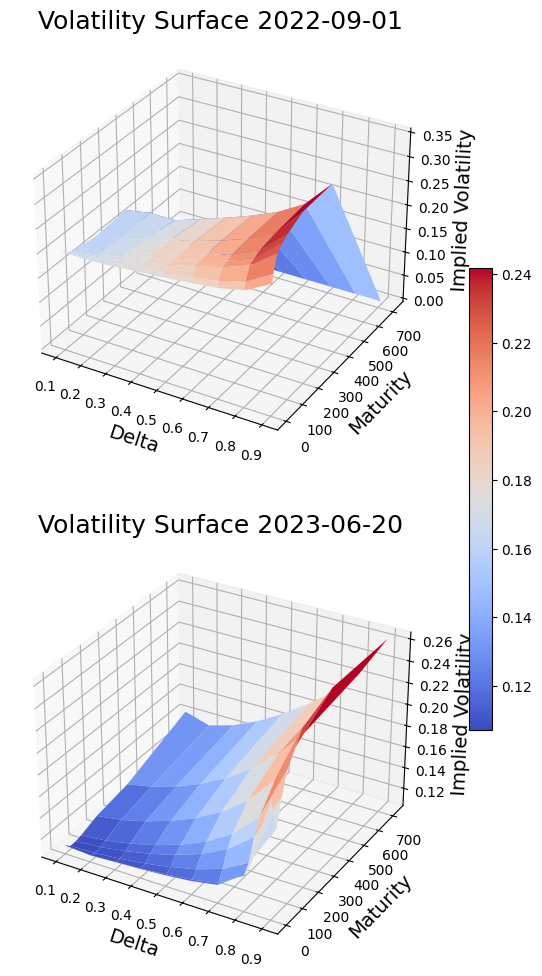
\includegraphics[width=0.65\linewidth]{docs/slides/img/vol_sample.png}
    \caption{DATASOURCE:WRDS}
    \label{fig:enter-label}
\end{figure}
DATASOURCE:WRDS
    \end{column}
\end{columns}

\end{frame}

% 2. VAE Theory Review
\begin{frame}{Variational Autoencoder (VAE): Review}
    \begin{figure}
    \centering
    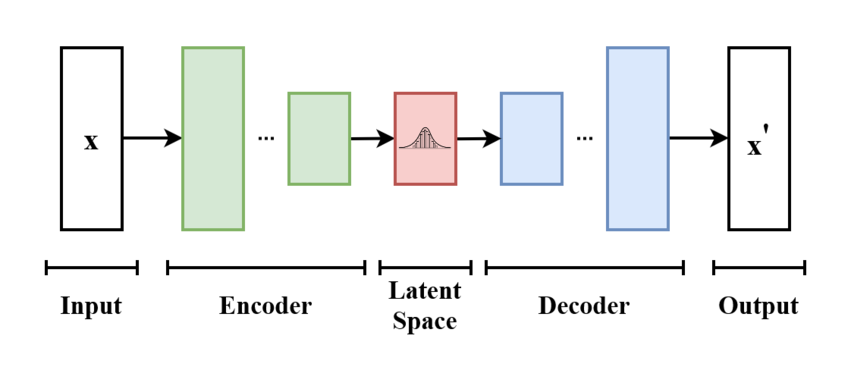
\includegraphics[width=0.6\linewidth]{docs/proposal/img/vaewiki.png}
    \caption{VAE architecture (source: Wikipedia)}
    \label{fig:vaewiki}
\end{figure}
\begin{itemize}
    \item Encoder: $q_\phi(\bf{z}\mid \bf{x})$ \quad Decoder: $p_\theta(\bf{x}\mid \bf{z})$

\end{itemize}
\textbf{Objective:} Maximize ELBO (Evidence Lower Bound):
\begin{align*}
\mathcal{L}(\theta, \phi) &= \mathbb{E}_{q_\phi(z|x)}[\log p_\theta(x|z)] - D_{\text{KL}}(q_\phi(z|x) \parallel p(z))\\
(\beta\text{-VAE})&\rightarrow \mathbb{E}_{q_\phi(z|x)}[\log p_\theta(x|z)] - \beta \cdot D_{\text{KL}}(q_\phi(z|x) \parallel p(z))
\end{align*}
\end{frame}


\begin{frame}{Variational Autoencoder (VAE): Review}

\begin{figure}
    \centering
    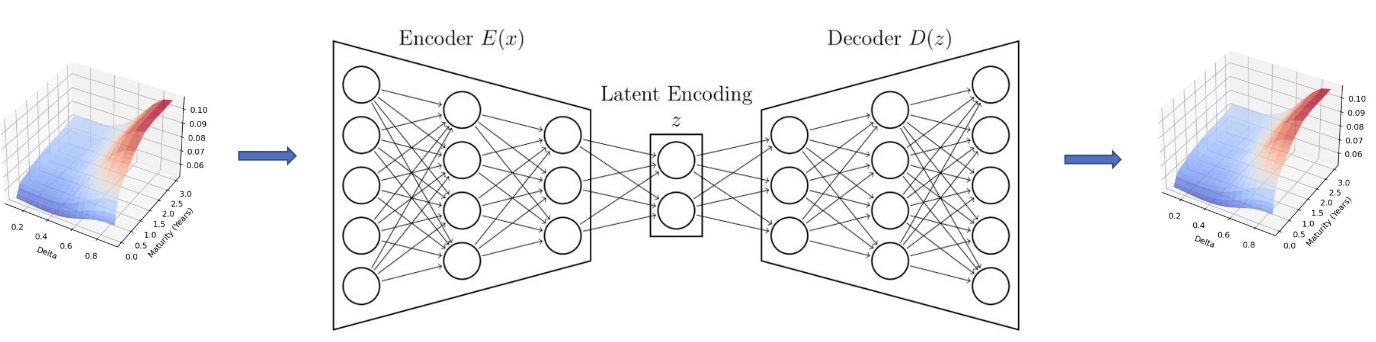
\includegraphics[width=0.85\linewidth]{docs/slides/img/model_design_full.png}
    \caption{Model Design}
\end{figure}

\begin{itemize}
    \item $\bf{z} \sim \mathcal{N}(0,\bf{1})$
    \item $\mathbf{z}\mid \mathbf{x}\sim \mathcal{N}(\mathbf{\mu}_\phi(x), \Sigma_\phi(x))$
\end{itemize}
\textbf{Minimize Loss Function:}
$$\mathcal{L}(\theta, \phi) = MSE(x, x') + \beta \cdot D_{\text{KL}}(q_\phi(z|x) \parallel p(z))$$
\end{frame}


\section{Models}

% 3. Model Architectures


\begin{frame}{Model Design: Grid-Based vs. Pointwise VAE}
\begin{columns}
    \begin{column}{0.6\textwidth}
\textbf{Input} for both encoders: \\ Entire volatility surface grid \(\mathbf{V} \in \mathbb{R}^{K \times T}\)
\vspace{0.3cm}

\textbf{Grid-Based VAE:}
\begin{itemize}
    \item Input for decoder: Latent variables $\bf{z}$
    \item Output: A grid surface
\end{itemize}
\textbf{Pointwise VAE (\citet{vaeorigin}):}
\begin{itemize}
    \item Input for decoder: $ (\mathbf{z}, K, T) $
    \item Output: A point $\sigma(T,K,z_1,...z_d)$
\end{itemize}
  \end{column}
  \begin{column}{0.4\textwidth}
    \begin{figure}
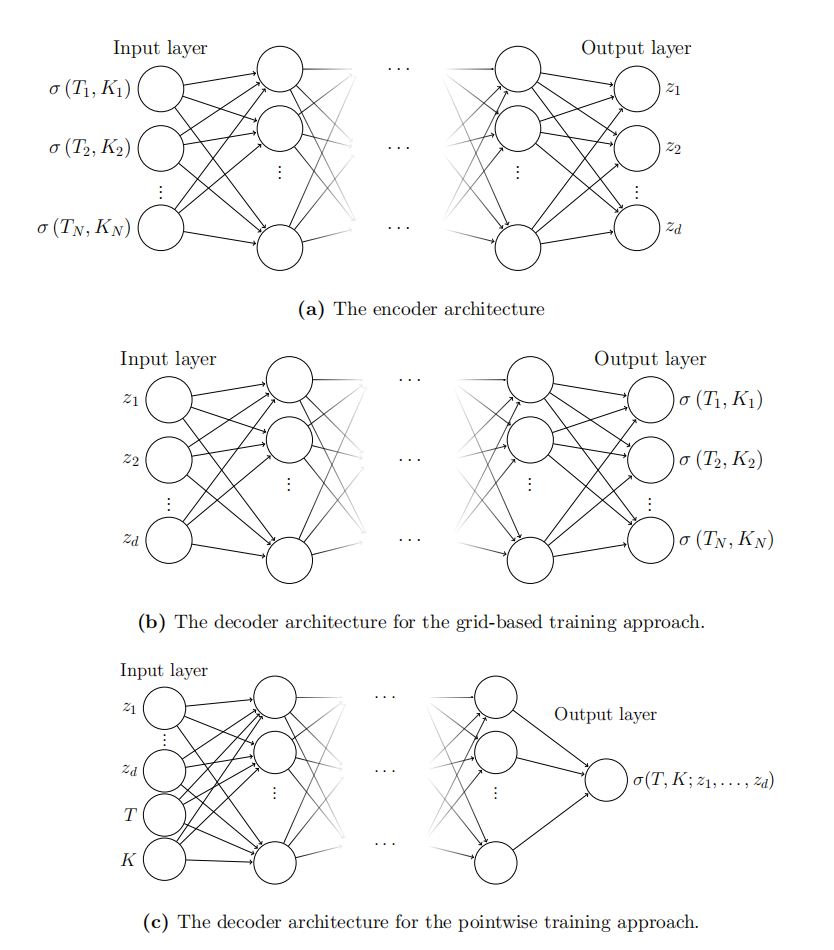
\includegraphics[width=\textwidth]{docs/slides/img/vae_vol.png}
\caption{Pointwise architecture.}
\end{figure}
  \end{column}
\end{columns}
\end{frame}
\begin{frame}{Usage: Grid-Based vs. Pointwise VAE}
\begin{columns}
    \begin{column}{0.48\textwidth}
        \textbf{Grid-Based VAE}
        \begin{itemize}
            \item Generate new volatility surface on grids.
            \item Stress tests.
            \item Latent space analysis.
        \end{itemize}
    \end{column}
    \begin{column}{0.48\textwidth}
    \textbf{Pointwise VAE}
\begin{itemize}
    \item Generate new volatility surface at any points.
    \item Predict missing points.
    \item Interpolation and extrapolation of the surface.
    \item Arbitrage.
\end{itemize}
    \end{column}
\end{columns}
\end{frame}

\begin{frame}{Model design: paper vs. us}
\begin{figure}
    \centering
    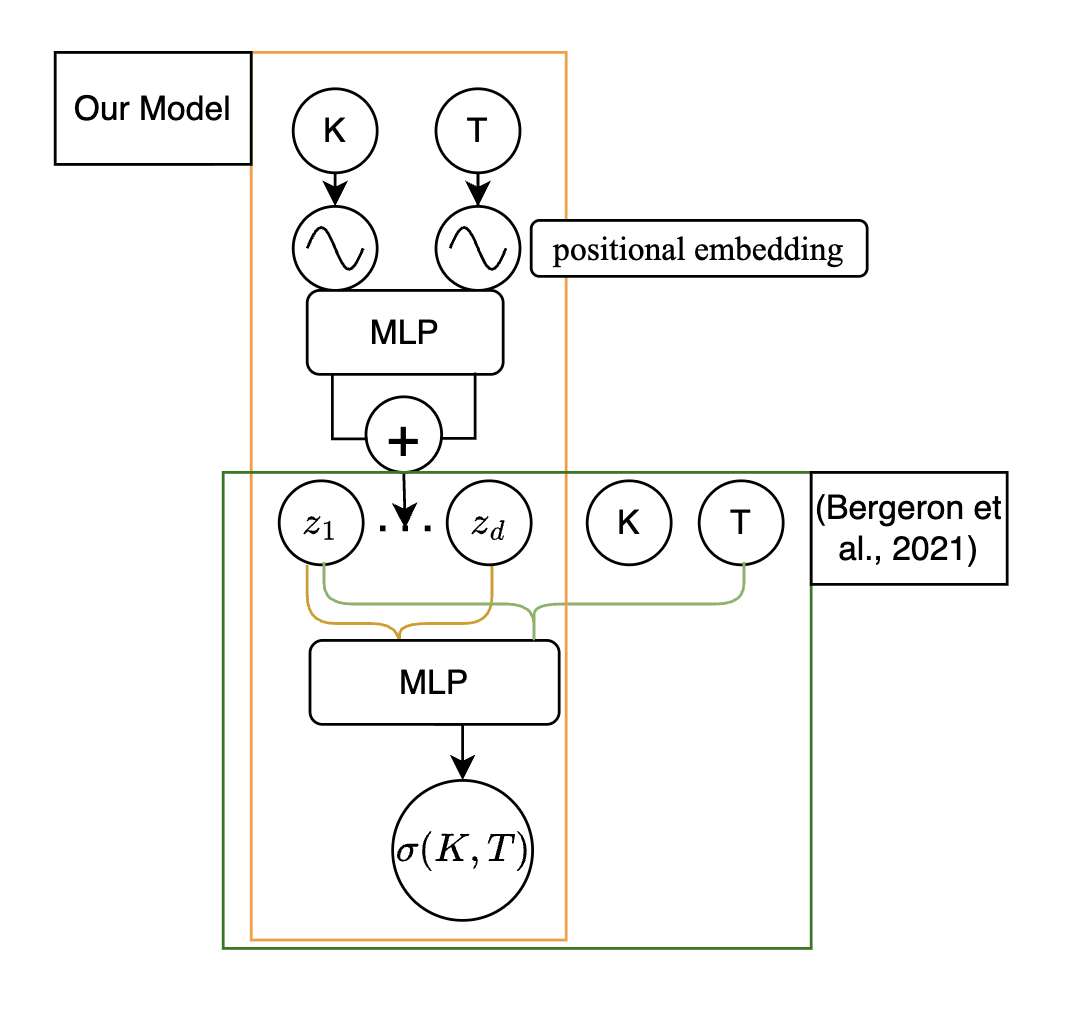
\includegraphics[width=0.65\linewidth]{docs/slides/img/model_design.png}
    \caption{Structure Comparison in Decoder}
    \label{fig:enter-label}
\end{figure}
    
\end{frame}


% % 4. Dataset
% \begin{frame}{Dataset: SPX Options from WRDS}
% \begin{itemize}
%     \item Source: Wharton Research Data Services (WRDS)
%     \item Spot: SPX Options
%     \item Time range: 08/31/2022 - 08/31/2023
%     \item Key statistics:
%     \begin{table}
%     \centering
%     \begin{tabular}{@{}ll@{}}
%     \toprule
%     Maturities & 1D–2Y \\
%     Data points & 1.2M (post-filtering) \\
%     \bottomrule
%     \end{tabular}
%     \end{table}
% \end{itemize}
% \begin{figure}
%     \centering
%     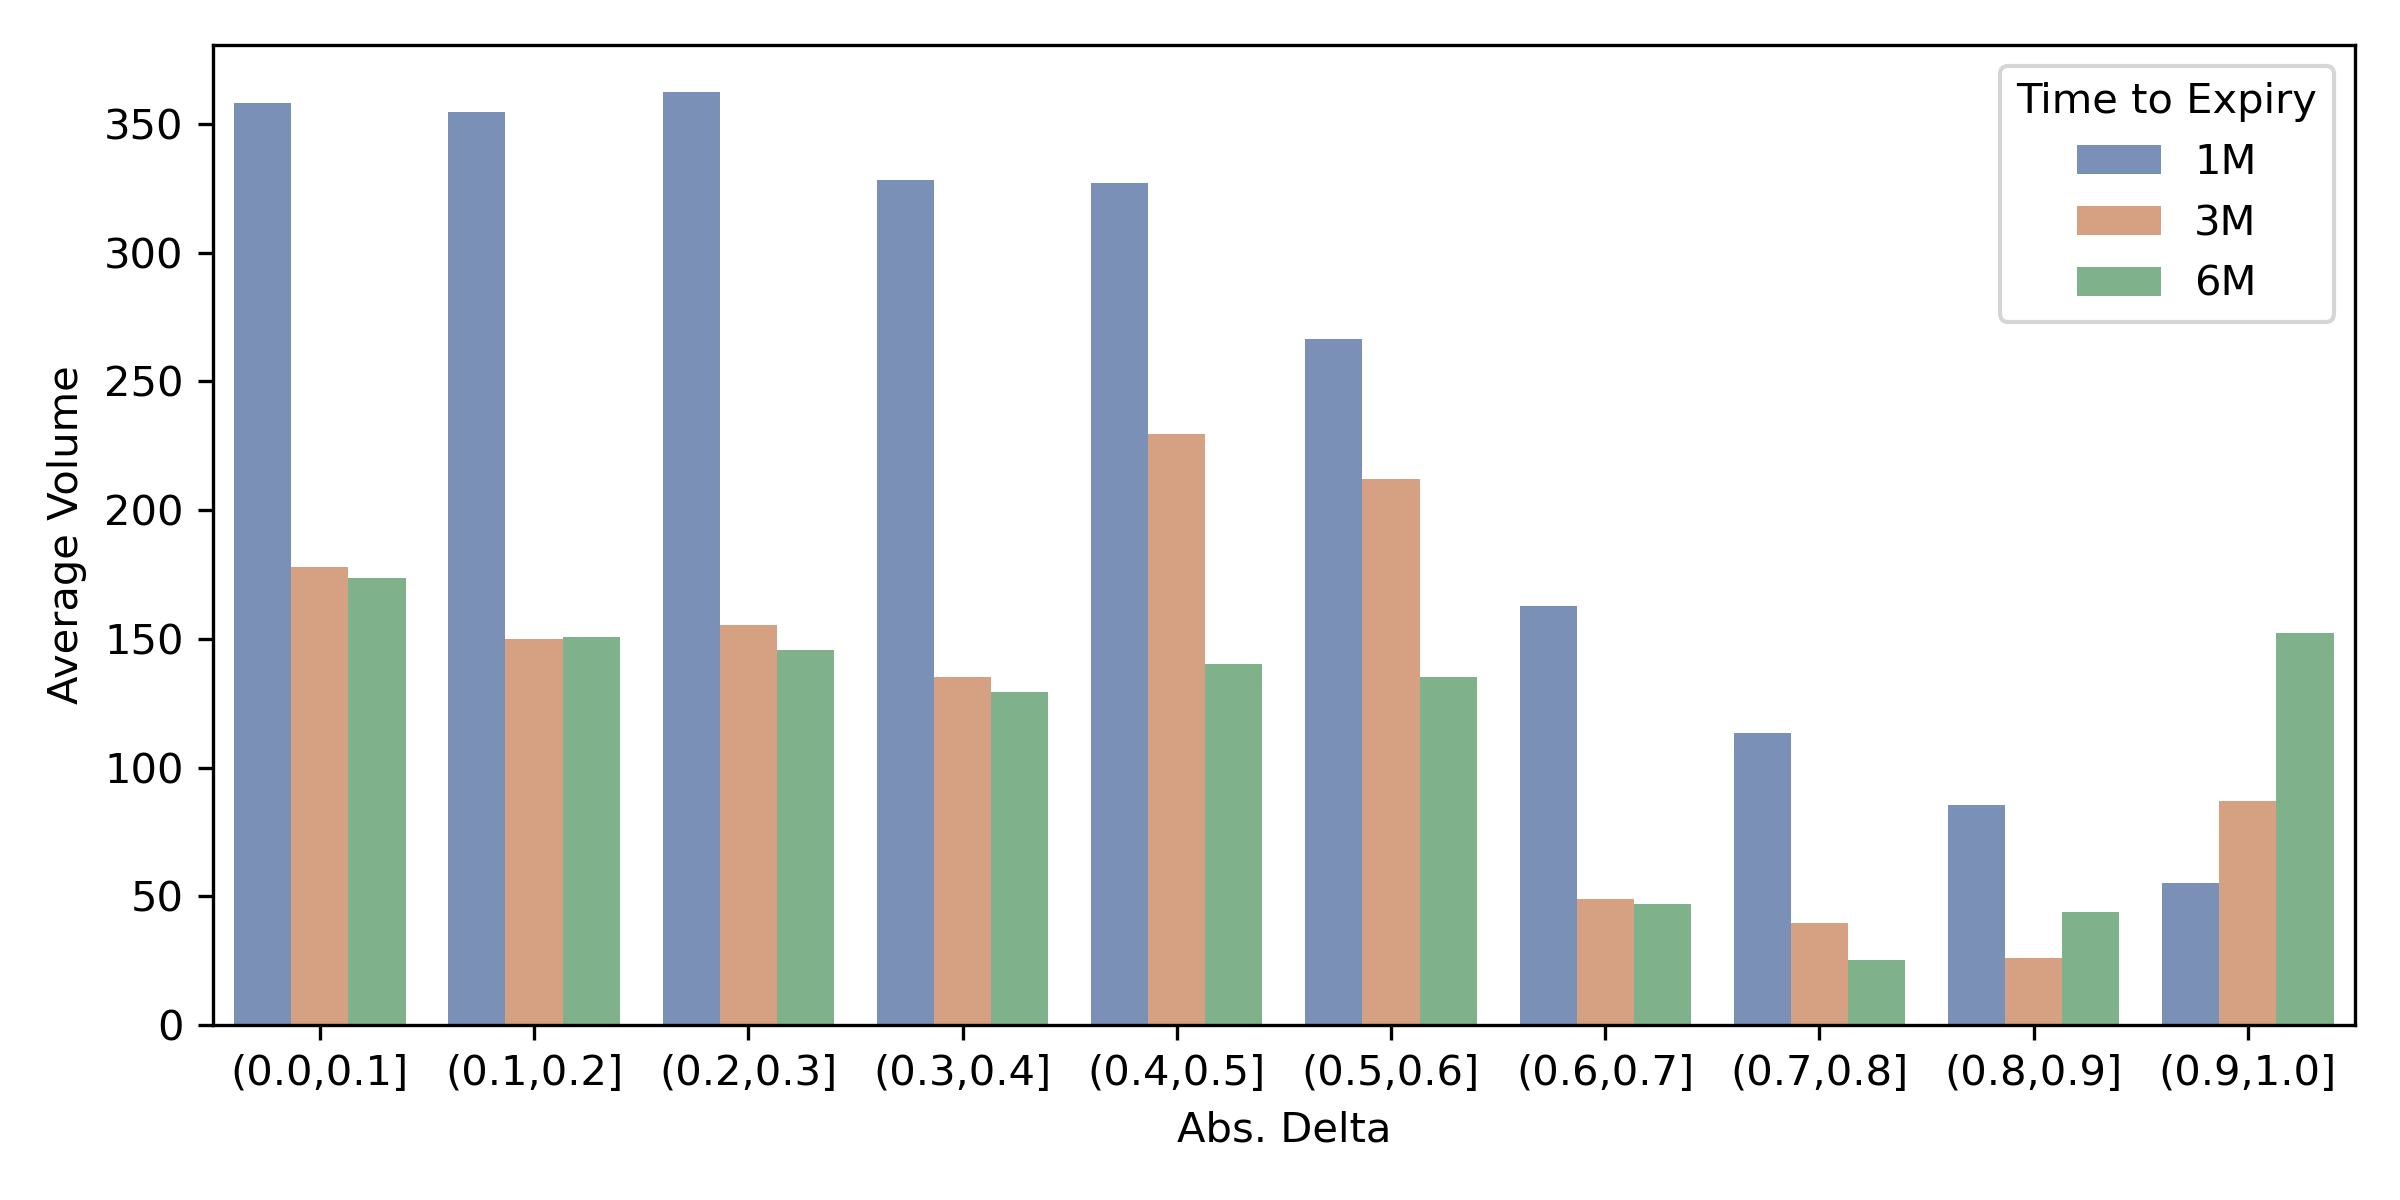
\includegraphics[width=0.5\linewidth]{docs/slides/img/vlm_by_delta_brackets.png}
%     \title{Average Volume by Delta Bracket}
% \end{figure}

% \end{frame}
\section{Experiments}
% 5. Results: VAE Generated Surfaces
\begin{frame}{VAE-Generated Volatility Surfaces}
\todo
some model: VAE generated, compare different latent dims
\end{frame}

\begin{frame}{VAE-Generated Volatility Surfaces}
Grid-Based
\end{frame}

\begin{frame}{VAE-Generated Volatility Surfaces}
\begin{figure}
    \centering
    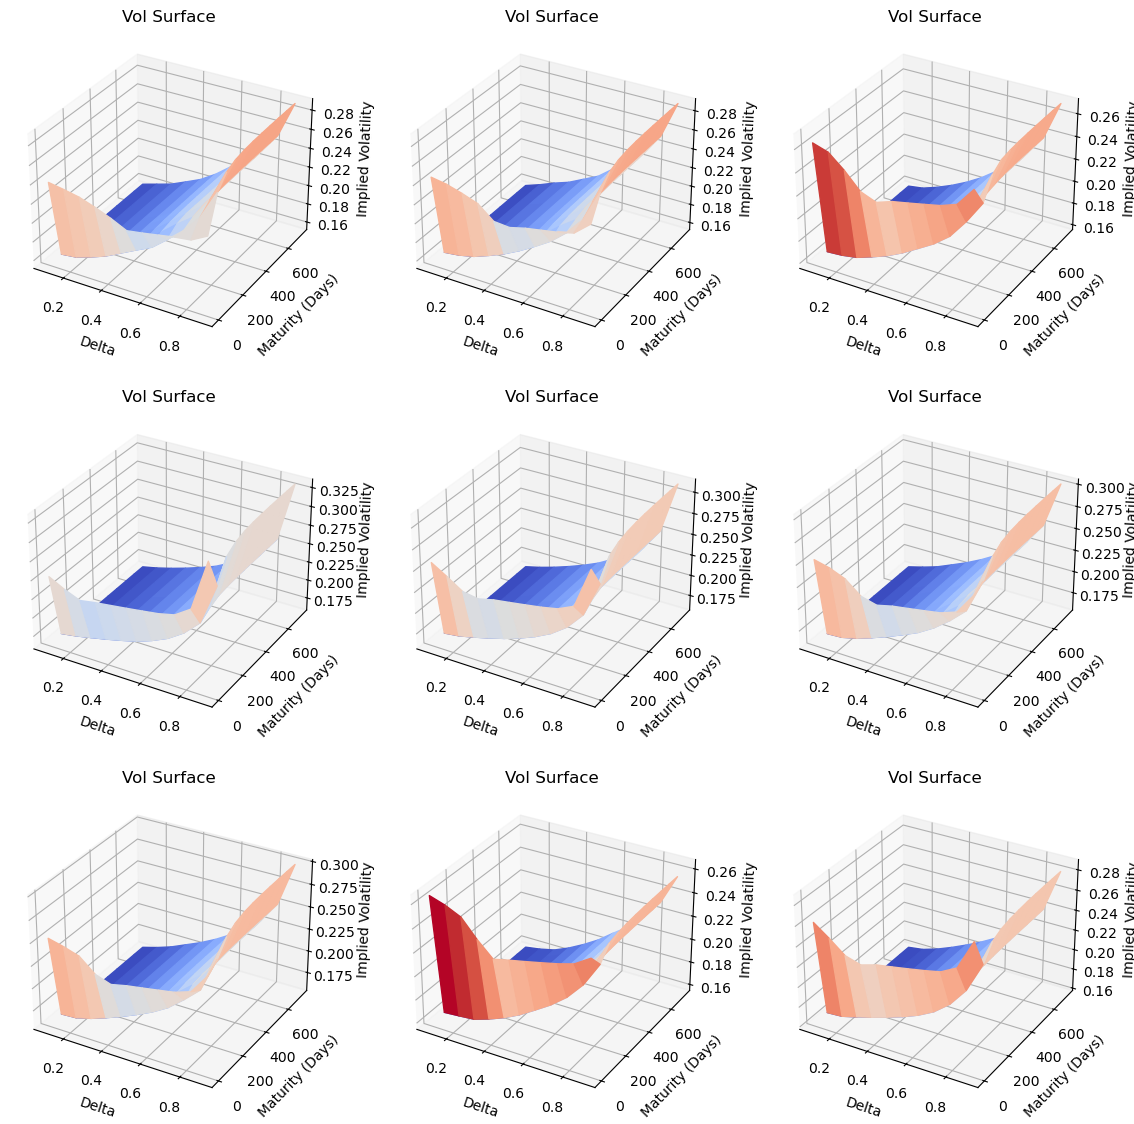
\includegraphics[width=0.65\linewidth]{docs/slides/img/vae_pw_ii_beta0.1.png}
    \caption{Structure Comparison in Decoder}
    \label{fig:enter-label}
\end{figure}
\end{frame}

% 6. Latent Space Analysis
\begin{frame}{Latent Space Visualization}
\begin{figure}
    \centering
    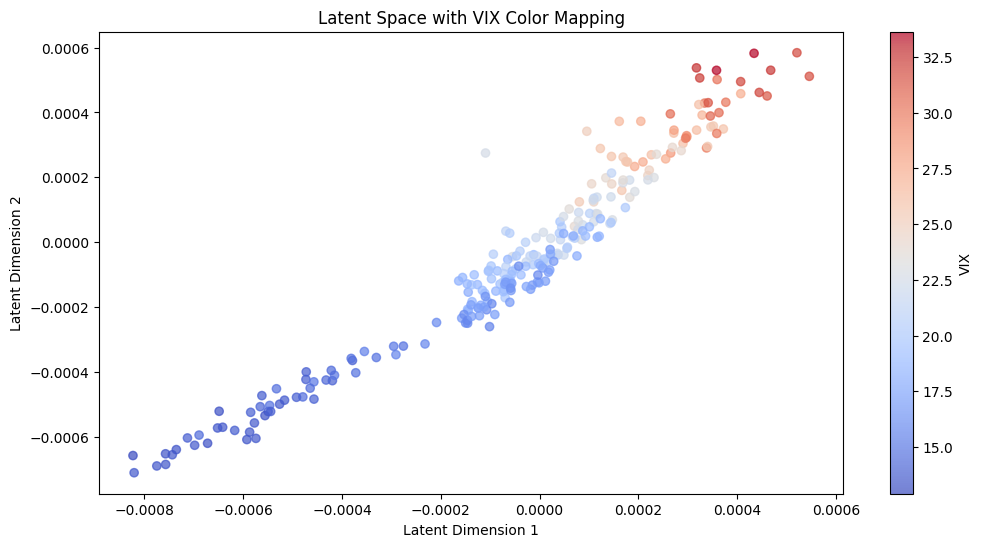
\includegraphics[width=0.8\linewidth]{docs/slides/img/latent.png}
    \caption{Latent $\bf{z}$ with VIX coloring}
    \label{fig:enter-label}
\end{figure}
\end{frame}

% 7. Pointwise VAE Performance
\begin{frame}{Pointwise VAE: Interpolation Results}
\todo
some figures for prediction

\end{frame}

% 8. Result Analysis
\begin{frame}{Key Advantages of VAE Approach}
\begin{itemize}
    \item \textbf{Flexibility}: Captures non-parametric volatility dynamics
    
    \item \textbf{Robustness}: Handles missing data via latent structure

    \item \textbf{Potential:} Predicting the shape of volatility surface.
\end{itemize}
\vspace{0.5cm}
\textbf{Limitations:}
\begin{itemize}
    \item Sensitive to hyperparameters (\(\beta\)-VAE trade-off)
    \item Interpretability vs. traditional models
\end{itemize}
\textbf{Key findings:}
\begin{itemize}
    \item Volatility surfaces might be controlled by latent variables with a small size.
    \item VAE might reduce the noise and extract some features in market data.
\end{itemize}
\end{frame}

% 9. Future Work
\begin{frame}{Future Directions}
\begin{itemize}
\item \textbf{Real-time Adaptation}: Online learning for regime shifts
    \item \textbf{Diffusion Models}: Add diffusion process in latent space (latent diffusion models) :
    \[
    q(x_{1:T}|x_0) = \prod_{t=1}^T q(x_t|x_{t-1}), \quad q(x_t|x_{t-1}) = \mathcal{N}(x_t; \sqrt{1-\beta_t}x_{t-1}, \beta_t \mathbf{I})
    \]
\begin{figure}
    \centering
    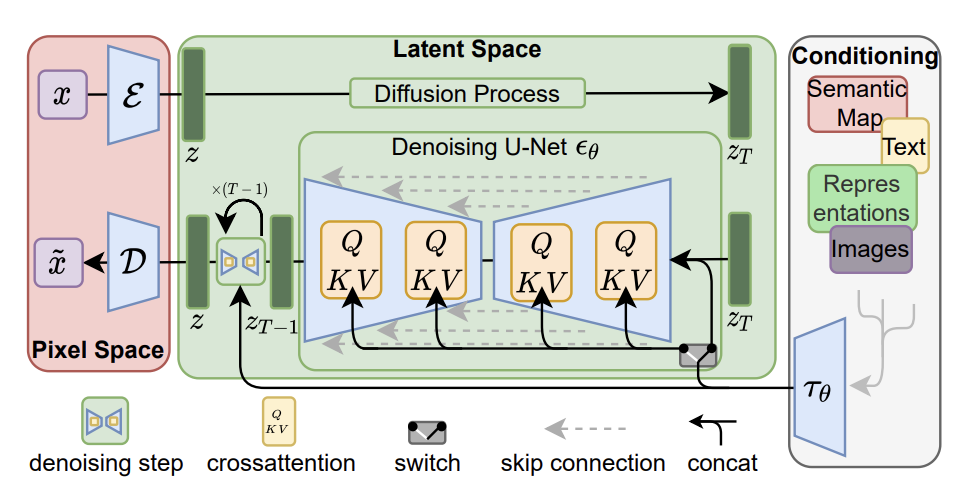
\includegraphics[width=0.6\linewidth]{docs/proposal/img/ldm.png}
    \caption{Latent Diffusion Models Structure}
    \label{fig:enter-label}
\end{figure}
\end{itemize}



\end{frame}

\begin{frame}{Reference}
    \bibliography{ref}
    
\end{frame}



\end{document}